\chapter{Cycles énergétiques}
\section{Cycle du soleil}

La Terre tourne autour du soleil en 365 jours et 8 heures, mais tourne aussi sur elle même en 24 heures.
Ce cycle de 24 heures, appelé le cycle jour-nuit, est influé par l'orientation de la Terre face au Soleil.
Son axe de rotation forme en effet un angle de 23° degrés avec le Soleil.

Suivant le pôle faisant face à l'étoile, l'ensoleillement diffère avec des extrêmes aux pôles où la nuit ne tombe
qu'une fois par an pour une durée de 6 mois.

Plus on s'approche de l'équateur, moins cet effet est ressenti. Cela a un impact fort sur les technologies
accessibles et utilisables par les différentes populations.

La rentabilité d'un panneau solaire est plus faible au pôles qu'à l'équateur.
En revanche, du fait des changements de température importants au long de l'année, les régions proches des pôles
sont propices au vent et donc aux énergies éoliennes.

La production est influencée par ce que l'on appelle la déclinaison solaire.
La déclinaison solaire $\delta$ correspond à l’angle que forme la direction
Terre-Soleil par rapport au plan de l’équateur terrestre.

L'équation suivante, avec J correspondant au jour de l'année, nous donne cette déclinaison.

% http://www.plevenon-meteo.info/technique/theorie/enso/ensoleillement.html
\begin{equation}
  \delta = 23.45 \times \sin \left( 360 \times \frac{284 + J}{365} \right)
\end{equation}


\section{Cycle circadien humain}
% cycles d’environ 24 heures
% Synchronisation par la lumiere du jour au niveaux de l’hypothamus
% le niveau de mélatonine sanguin est très faible le jour
% Plus la lumière diminue d’intensité, plus ce niveau augmente pour atteindre un degré maximal de sécrétion entre deux et quatre heures du matin

% Le cycle est different en fonction de l'age
% Newborn babies: They still don’t have a well formed circadian cycle, that’s the reason why they sleep on and off. As their sleep cycle gets more consolidated, daytime naps are less frequent and sleep is consolidated during the night.
% Children: Children need more sleep than adults, 11-13 hours per night between age 3-5 and 10-11 hours between 6 and 9 years old.
% Teenagers: Hormonal shifts change the circadian rhythm, making them go to bed later at night, and waking them up later in the morning.
% Adults: Adults needs between 7-9 hours of sleep every night. Some lifestyle choices, such as consumption of caffeine, stress and screen use during the evening disrupt our sleep cycle.


% Activitees pouvant de-regler le cycle :
% - Blue LED lightning, commonly emitted by screens, reduces melatonin production. This impacts our ability to fall asleep. We strongly encourage you to use blue light filters during the evening .
% - Travail de nuit

% Sources
% https://fondationsommeil.com/le-cycle-circadien/
% https://en.getmoona.com/blogs/mission-sleep/how-your-circadian-rhythm-influences-your-sleep


Le rythme circadien est un processus naturel et interne qui régule le cycle
veille-sommeil et se répète à peu près toutes les 24 heures.
Il peut se référer à tout processus biologique qui présente une oscillation
endogène et entraînable d'environ 24 heures.

\begin{figure}[h]
  \centering
  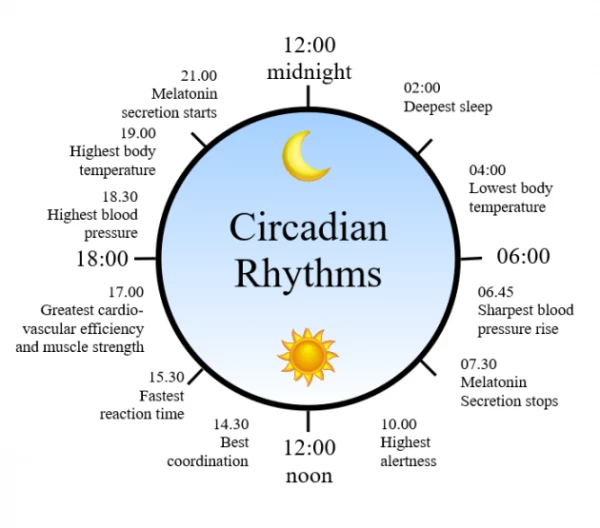
\includegraphics[scale=2.0]{media/circadien.png}
  \caption{
      Les cycles du rythme circadien\newline
      \tiny{Source: \url{https://en.getmoona.com/blogs/mission-sleep/how-your-circadian-rhythm-influences-your-sleep}}
  }
\end{figure}

La rythmicité circadienne est présente dans les habitudes de sommeil et
d'alimentation des animaux, y compris des êtres humains. Il existe également
des schémas clairs de température corporelle centrale, d'activité des ondes cérébrales,
de production d'hormones, de régénération cellulaire et d'autres activités biologiques.
En outre, le photopériodisme, la réaction physiologique des organismes à la longueur du
jour ou de la nuit, est vital pour les plantes et les animaux, et le système circadien
joue un rôle dans la mesure et l'interprétation de la longueur du jour.

La prévision en temps utile des périodes saisonnières de conditions météorologiques,
de disponibilité de la nourriture ou d'activité des prédateurs est cruciale pour
la survie de nombreuses espèces.

La perturbation des cycles du sommeil provoque des troubles de sommeil.
Le travailleur de nuit est particulièrement à risque et n’obtient souvent
pas tous les bienfaits d’un sommeil réparateur, car ces cycles sont perturbés
notamment par l’incapacité du système à s’adapter à une routine de sommeil spécifique.

\section{Cycles long cours}
% Cette partie parlera des differents cycles terrestres prenant cours sur le long terme
% ex. Courants marins - Point chaud

Sur Terre, de nombreux cycles sont à des échelles plus grandes.

Les différents courants marins tel que le golf stream n'éxistaient pas il y a 10 000 ans, et commencent à faiblir.

Quand le point chaud se situe sous l'océan, la lenteur de l'écoulement provoque une accumulation de
lave qui refroidit au contact de l'eau et forme alors des îles volcaniques.

L'Islande et la Réunion sont des exemples d'îles volcaniques de ce genre.
On sait depuis près d'un siècle que les plaques tectoniques sont en perpétuel mouvement.

Les plaques tectoniques déplacent les continents à raison de 5 cm par an. C'est un changement infime
qui à produit l'Archipel des Caraïbes. Un point chaud, résultant d'une chaleur du centre de la Terre,
reste en effet statique et produit une nouvelle île.

Ces différents cycles imposent à l'Homme de les prendre en compte dans leurs déploiements d'utilisation de l'énergie.

L'affaiblissement du Golf Stream rend inintéressant l'exploitation de celui-ci par des hydroliennes contrairement
à ce que les mesures des précédentes années montraient.

% Mettre une image de la chute de vitesse du golf stream

\section{Équilibre de la production}

Du fait de ces déséquilibres géographiques, il n'est pas possible de compter sur la même source d'énergie partout
sur le globe, il va falloir équilibrer la production aux différentes sources locales.

Les régions insulaires sont riches en volcans. Or la géothermie est un moyen simple d'utiliser cette énergie.
Les régions proches des tropiques profitent d'un anti-cyclone permanent et d'un ensoleillement
idéal pour la technologie solaire, à condition d'améliorer l'efficacité de celle-ci lors de fortes températures.

\section{Anticipation de la production}

Il est possible d'anticiper la production à condition de connaître toutes les sources d'énergies
exploités dans un cluster donné.

Si par exemple la zone est équipée de panneaux solaires, on peut estimer sa production à l'aide de
l'ensoleillement et de la couverture nuageuse.

L'ensoleillement est facile à mesurer. Les satellites en orbite de la Terre parviennent à l'indiquer à la minute près
des mois à l'avance.
Il est plus difficile en revanche de prédire la couverture nuageuse de l'année due au chaos qu'est le climat.
